\documentclass[1p]{elsarticle_modified}
%\bibliographystyle{elsarticle-num}

%\usepackage[colorlinks]{hyperref}
%\usepackage{abbrmath_seonhwa} %\Abb, \Ascr, \Acal ,\Abf, \Afrak
\usepackage{amsfonts}
\usepackage{amssymb}
\usepackage{amsmath}
\usepackage{amsthm}
\usepackage{scalefnt}
\usepackage{amsbsy}
\usepackage{kotex}
\usepackage{caption}
\usepackage{subfig}
\usepackage{color}
\usepackage{graphicx}
\usepackage{xcolor} %% white, black, red, green, blue, cyan, magenta, yellow
\usepackage{float}
\usepackage{setspace}
\usepackage{hyperref}

\usepackage{tikz}
\usetikzlibrary{arrows}

\usepackage{multirow}
\usepackage{array} % fixed length table
\usepackage{hhline}

%%%%%%%%%%%%%%%%%%%%%
\makeatletter
\renewcommand*\env@matrix[1][\arraystretch]{%
	\edef\arraystretch{#1}%
	\hskip -\arraycolsep
	\let\@ifnextchar\new@ifnextchar
	\array{*\c@MaxMatrixCols c}}
\makeatother %https://tex.stackexchange.com/questions/14071/how-can-i-increase-the-line-spacing-in-a-matrix
%%%%%%%%%%%%%%%

\usepackage[normalem]{ulem}

\newcommand{\msout}[1]{\ifmmode\text{\sout{\ensuremath{#1}}}\else\sout{#1}\fi}
%SOURCE: \msout is \stkout macro in https://tex.stackexchange.com/questions/20609/strikeout-in-math-mode

\newcommand{\cancel}[1]{
	\ifmmode
	{\color{red}\msout{#1}}
	\else
	{\color{red}\sout{#1}}
	\fi
}

\newcommand{\add}[1]{
	{\color{blue}\uwave{#1}}
}

\newcommand{\replace}[2]{
	\ifmmode
	{\color{red}\msout{#1}}{\color{blue}\uwave{#2}}
	\else
	{\color{red}\sout{#1}}{\color{blue}\uwave{#2}}
	\fi
}

\newcommand{\Sol}{\mathcal{S}} %segment
\newcommand{\D}{D} %diagram
\newcommand{\A}{\mathcal{A}} %arc


%%%%%%%%%%%%%%%%%%%%%%%%%%%%%5 test

\def\sl{\operatorname{\textup{SL}}(2,\Cbb)}
\def\psl{\operatorname{\textup{PSL}}(2,\Cbb)}
\def\quan{\mkern 1mu \triangleright \mkern 1mu}

\theoremstyle{definition}
\newtheorem{thm}{Theorem}[section]
\newtheorem{prop}[thm]{Proposition}
\newtheorem{lem}[thm]{Lemma}
\newtheorem{ques}[thm]{Question}
\newtheorem{cor}[thm]{Corollary}
\newtheorem{defn}[thm]{Definition}
\newtheorem{exam}[thm]{Example}
\newtheorem{rmk}[thm]{Remark}
\newtheorem{alg}[thm]{Algorithm}

\newcommand{\I}{\sqrt{-1}}
\begin{document}

%\begin{frontmatter}
%
%\title{Boundary parabolic representations of knots up to 8 crossings}
%
%%% Group authors per affiliation:
%\author{Yunhi Cho} 
%\address{Department of Mathematics, University of Seoul, Seoul, Korea}
%\ead{yhcho@uos.ac.kr}
%
%
%\author{Seonhwa Kim} %\fnref{s_kim}}
%\address{Center for Geometry and Physics, Institute for Basic Science, Pohang, 37673, Korea}
%\ead{ryeona17@ibs.re.kr}
%
%\author{Hyuk Kim}
%\address{Department of Mathematical Sciences, Seoul National University, Seoul 08826, Korea}
%\ead{hyukkim@snu.ac.kr}
%
%\author{Seokbeom Yoon}
%\address{Department of Mathematical Sciences, Seoul National University, Seoul, 08826,  Korea}
%\ead{sbyoon15@snu.ac.kr}
%
%\begin{abstract}
%We find all boundary parabolic representation of knots up to 8 crossings.
%
%\end{abstract}
%\begin{keyword}
%    \MSC[2010] 57M25 
%\end{keyword}
%
%\end{frontmatter}

%\linenumbers
%\tableofcontents
%
\newcommand\colored[1]{\textcolor{white}{\rule[-0.35ex]{0.8em}{1.4ex}}\kern-0.8em\color{red} #1}%
%\newcommand\colored[1]{\textcolor{white}{ #1}\kern-2.17ex	\textcolor{white}{ #1}\kern-1.81ex	\textcolor{white}{ #1}\kern-2.15ex\color{red}#1	}

{\Large $\underline{12n_{0190}~(K12n_{0190})}$}

\setlength{\tabcolsep}{10pt}
\renewcommand{\arraystretch}{1.6}
\vspace{1cm}\begin{tabular}{m{100pt}>{\centering\arraybackslash}m{274pt}}
\multirow{5}{120pt}{
	\centering
	\includegraphics[width=112pt]{../../../GIT/diagram.site/Diagrams/png/2279_12n_0190.png}\\
\ \ \ A knot diagram\footnotemark}&
\allowdisplaybreaks
\textbf{Linearized knot diagam} \\
\cline{2-2}
 &
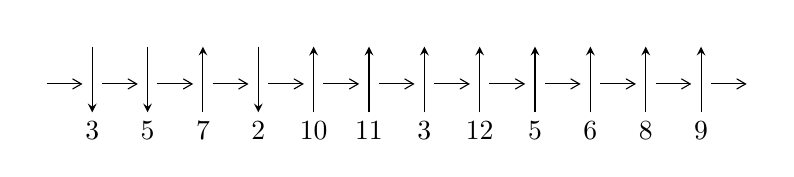
\begin{tikzpicture}[x=20pt, y=17pt]
	% nodes
	\node (C0) at (0, 0) {};
	\node (C1) at (1, 0) {};
	\node (C1U) at (1, +1) {};
	\node (C1D) at (1, -1) {3};

	\node (C2) at (2, 0) {};
	\node (C2U) at (2, +1) {};
	\node (C2D) at (2, -1) {5};

	\node (C3) at (3, 0) {};
	\node (C3U) at (3, +1) {};
	\node (C3D) at (3, -1) {7};

	\node (C4) at (4, 0) {};
	\node (C4U) at (4, +1) {};
	\node (C4D) at (4, -1) {2};

	\node (C5) at (5, 0) {};
	\node (C5U) at (5, +1) {};
	\node (C5D) at (5, -1) {10};

	\node (C6) at (6, 0) {};
	\node (C6U) at (6, +1) {};
	\node (C6D) at (6, -1) {11};

	\node (C7) at (7, 0) {};
	\node (C7U) at (7, +1) {};
	\node (C7D) at (7, -1) {3};

	\node (C8) at (8, 0) {};
	\node (C8U) at (8, +1) {};
	\node (C8D) at (8, -1) {12};

	\node (C9) at (9, 0) {};
	\node (C9U) at (9, +1) {};
	\node (C9D) at (9, -1) {5};

	\node (C10) at (10, 0) {};
	\node (C10U) at (10, +1) {};
	\node (C10D) at (10, -1) {6};

	\node (C11) at (11, 0) {};
	\node (C11U) at (11, +1) {};
	\node (C11D) at (11, -1) {8};

	\node (C12) at (12, 0) {};
	\node (C12U) at (12, +1) {};
	\node (C12D) at (12, -1) {9};
	\node (C13) at (13, 0) {};

	% arrows
	\draw[->,>={angle 60}]
	(C0) edge (C1) (C1) edge (C2) (C2) edge (C3) (C3) edge (C4) (C4) edge (C5) (C5) edge (C6) (C6) edge (C7) (C7) edge (C8) (C8) edge (C9) (C9) edge (C10) (C10) edge (C11) (C11) edge (C12) (C12) edge (C13) ;	\draw[->,>=stealth]
	(C1U) edge (C1D) (C2U) edge (C2D) (C3D) edge (C3U) (C4U) edge (C4D) (C5D) edge (C5U) (C6D) edge (C6U) (C7D) edge (C7U) (C8D) edge (C8U) (C9D) edge (C9U) (C10D) edge (C10U) (C11D) edge (C11U) (C12D) edge (C12U) ;
	\end{tikzpicture} \\
\hhline{~~} \\& 
\textbf{Solving Sequence} \\ \cline{2-2} 
 &
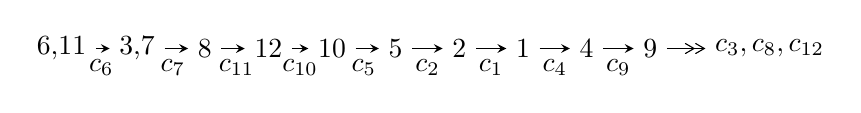
\begin{tikzpicture}[x=23pt, y=7pt]
	% node
	\node (A0) at (-1/8, 0) {6,11};
	\node (A1) at (17/16, 0) {3,7};
	\node (A2) at (17/8, 0) {8};
	\node (A3) at (25/8, 0) {12};
	\node (A4) at (33/8, 0) {10};
	\node (A5) at (41/8, 0) {5};
	\node (A6) at (49/8, 0) {2};
	\node (A7) at (57/8, 0) {1};
	\node (A8) at (65/8, 0) {4};
	\node (A9) at (73/8, 0) {9};
	\node (C1) at (1/2, -1) {$c_{6}$};
	\node (C2) at (13/8, -1) {$c_{7}$};
	\node (C3) at (21/8, -1) {$c_{11}$};
	\node (C4) at (29/8, -1) {$c_{10}$};
	\node (C5) at (37/8, -1) {$c_{5}$};
	\node (C6) at (45/8, -1) {$c_{2}$};
	\node (C7) at (53/8, -1) {$c_{1}$};
	\node (C8) at (61/8, -1) {$c_{4}$};
	\node (C9) at (69/8, -1) {$c_{9}$};
	\node (A10) at (11, 0) {$c_{3},c_{8},c_{12}$};

	% edge
	\draw[->,>=stealth]	
	(A0) edge (A1) (A1) edge (A2) (A2) edge (A3) (A3) edge (A4) (A4) edge (A5) (A5) edge (A6) (A6) edge (A7) (A7) edge (A8) (A8) edge (A9) ;
	\draw[->>,>={angle 60}]	
	(A9) edge (A10);
\end{tikzpicture} \\ 

\end{tabular} \\

\footnotetext{
The image of knot diagram is generated by the software ``\textbf{Draw programme}" developed by Andrew Bartholomew(\url{http://www.layer8.co.uk/maths/draw/index.htm\#Running-draw}), where we modified some parts for our purpose(\url{https://github.com/CATsTAILs/LinksPainter}).
}\phantom \\ \newline 
\centering \textbf{Ideals for irreducible components\footnotemark of $X_{\text{par}}$} 
 
\begin{align*}
I^u_{1}&=\langle 
9.44661\times10^{16} u^{34}-2.08351\times10^{16} u^{33}+\cdots+1.06489\times10^{17} b-4.51309\times10^{16},\\
\phantom{I^u_{1}}&\phantom{= \langle  }1.88308\times10^{16} u^{34}-8.66830\times10^{16} u^{33}+\cdots+1.06489\times10^{17} a-2.62684\times10^{17},\;u^{35}-2 u^{34}+\cdots-3 u^2+1\rangle \\
I^u_{2}&=\langle 
b+u+1,\;u^2+a-3,\;u^3+u^2-2 u-1\rangle \\
\\
\end{align*}
\raggedright * 2 irreducible components of $\dim_{\mathbb{C}}=0$, with total 38 representations.\\
\footnotetext{All coefficients of polynomials are rational numbers. But the coefficients are sometimes approximated in decimal forms when there is not enough margin.}
\newpage
\renewcommand{\arraystretch}{1}
\centering \section*{I. $I^u_{1}= \langle 9.45\times10^{16} u^{34}-2.08\times10^{16} u^{33}+\cdots+1.06\times10^{17} b-4.51\times10^{16},\;1.88\times10^{16} u^{34}-8.67\times10^{16} u^{33}+\cdots+1.06\times10^{17} a-2.63\times10^{17},\;u^{35}-2 u^{34}+\cdots-3 u^2+1 \rangle$}
\flushleft \textbf{(i) Arc colorings}\\
\begin{tabular}{m{7pt} m{180pt} m{7pt} m{180pt} }
\flushright $a_{6}=$&$\begin{pmatrix}1\\0\end{pmatrix}$ \\
\flushright $a_{11}=$&$\begin{pmatrix}0\\u\end{pmatrix}$ \\
\flushright $a_{3}=$&$\begin{pmatrix}-0.176834 u^{34}+0.814012 u^{33}+\cdots+2.45226 u+2.46678\\-0.887101 u^{34}+0.195656 u^{33}+\cdots+0.405852 u+0.423810\end{pmatrix}$ \\
\flushright $a_{7}=$&$\begin{pmatrix}1\\- u^2\end{pmatrix}$ \\
\flushright $a_{8}=$&$\begin{pmatrix}0.833303 u^{34}-1.64324 u^{33}+\cdots-2.63958 u+0.00424027\\0.474997 u^{34}-0.230903 u^{33}+\cdots-0.0819582 u-0.627396\end{pmatrix}$ \\
\flushright $a_{12}=$&$\begin{pmatrix}-0.772238 u^{34}+1.25159 u^{33}+\cdots+1.49520 u+0.508098\\-0.536061 u^{34}+0.622559 u^{33}+\cdots+1.22634 u+0.115057\end{pmatrix}$ \\
\flushright $a_{10}=$&$\begin{pmatrix}- u\\u\end{pmatrix}$ \\
\flushright $a_{5}=$&$\begin{pmatrix}- u^2+1\\u^2\end{pmatrix}$ \\
\flushright $a_{2}=$&$\begin{pmatrix}0.120048 u^{34}+0.252095 u^{33}+\cdots+2.07998 u+1.70401\\-0.898177 u^{34}+0.117584 u^{33}+\cdots+0.120048 u+0.492190\end{pmatrix}$ \\
\flushright $a_{1}=$&$\begin{pmatrix}1.16760 u^{34}-1.53977 u^{33}+\cdots-3.05490 u-0.519586\\0.247602 u^{34}-0.512958 u^{33}+\cdots-0.499946 u-0.126931\end{pmatrix}$ \\
\flushright $a_{4}=$&$\begin{pmatrix}-0.374572 u^{34}+1.04071 u^{33}+\cdots+3.03494 u+2.43025\\-0.739813 u^{34}+0.0918438 u^{33}+\cdots+0.208114 u+0.255027\end{pmatrix}$ \\
\flushright $a_{9}=$&$\begin{pmatrix}u^3-2 u\\- u^3+u\end{pmatrix}$\\&\end{tabular}
\flushleft \textbf{(ii) Obstruction class $= -1$}\\~\\
\flushleft \textbf{(iii) Cusp Shapes $= -\frac{218803516467230358}{106488603430183673} u^{34}+\frac{323482212694991959}{106488603430183673} u^{33}+\cdots+\frac{611689066048825845}{106488603430183673} u+\frac{1479659137766380195}{106488603430183673}$}\\~\\
\newpage\renewcommand{\arraystretch}{1}
\flushleft \textbf{(iv) u-Polynomials at the component}\newline \\
\begin{tabular}{m{50pt}|m{274pt}}
Crossings & \hspace{64pt}u-Polynomials at each crossing \\
\hline $$\begin{aligned}c_{1}\end{aligned}$$&$\begin{aligned}
&u^{35}+34 u^{34}+\cdots+115 u+1
\end{aligned}$\\
\hline $$\begin{aligned}c_{2},c_{4}\end{aligned}$$&$\begin{aligned}
&u^{35}-4 u^{34}+\cdots+11 u-1
\end{aligned}$\\
\hline $$\begin{aligned}c_{3},c_{7}\end{aligned}$$&$\begin{aligned}
&u^{35}-3 u^{34}+\cdots-68 u+8
\end{aligned}$\\
\hline $$\begin{aligned}c_{5},c_{6},c_{9}\\c_{10}\end{aligned}$$&$\begin{aligned}
&u^{35}+2 u^{34}+\cdots+3 u^2-1
\end{aligned}$\\
\hline $$\begin{aligned}c_{8},c_{11},c_{12}\end{aligned}$$&$\begin{aligned}
&u^{35}-2 u^{34}+\cdots+4 u-1
\end{aligned}$\\
\hline
\end{tabular}\\~\\
\newpage\renewcommand{\arraystretch}{1}
\flushleft \textbf{(v) Riley Polynomials at the component}\newline \\
\begin{tabular}{m{50pt}|m{274pt}}
Crossings & \hspace{64pt}Riley Polynomials at each crossing \\
\hline $$\begin{aligned}c_{1}\end{aligned}$$&$\begin{aligned}
&y^{35}-62 y^{34}+\cdots+24691 y-1
\end{aligned}$\\
\hline $$\begin{aligned}c_{2},c_{4}\end{aligned}$$&$\begin{aligned}
&y^{35}-34 y^{34}+\cdots+115 y-1
\end{aligned}$\\
\hline $$\begin{aligned}c_{3},c_{7}\end{aligned}$$&$\begin{aligned}
&y^{35}+21 y^{34}+\cdots+3536 y-64
\end{aligned}$\\
\hline $$\begin{aligned}c_{5},c_{6},c_{9}\\c_{10}\end{aligned}$$&$\begin{aligned}
&y^{35}-36 y^{34}+\cdots+6 y-1
\end{aligned}$\\
\hline $$\begin{aligned}c_{8},c_{11},c_{12}\end{aligned}$$&$\begin{aligned}
&y^{35}-24 y^{34}+\cdots+6 y-1
\end{aligned}$\\
\hline
\end{tabular}\\~\\
\newpage\flushleft \textbf{(vi) Complex Volumes and Cusp Shapes}
$$\begin{array}{c|c|c}  
\text{Solutions to }I^u_{1}& \I (\text{vol} + \sqrt{-1}CS) & \text{Cusp shape}\\
 \hline 
\begin{aligned}
u &= -0.518512 + 0.839070 I \\
a &= -0.20090 - 1.52795 I \\
b &= \phantom{-}0.503396 + 0.528590 I\end{aligned}
 & -5.06245 - 8.93378 I & \phantom{-}5.61011 + 6.33790 I \\ \hline\begin{aligned}
u &= -0.518512 - 0.839070 I \\
a &= -0.20090 + 1.52795 I \\
b &= \phantom{-}0.503396 - 0.528590 I\end{aligned}
 & -5.06245 + 8.93378 I & \phantom{-}5.61011 - 6.33790 I \\ \hline\begin{aligned}
u &= \phantom{-}0.555627 + 0.849121 I \\
a &= -0.614318 + 1.234160 I \\
b &= \phantom{-}0.699304 - 0.374906 I\end{aligned}
 & -9.19263 + 2.79140 I & \phantom{-}2.44794 - 2.71252 I \\ \hline\begin{aligned}
u &= \phantom{-}0.555627 - 0.849121 I \\
a &= -0.614318 - 1.234160 I \\
b &= \phantom{-}0.699304 + 0.374906 I\end{aligned}
 & -9.19263 - 2.79140 I & \phantom{-}2.44794 + 2.71252 I \\ \hline\begin{aligned}
u &= -0.602141 + 0.838097 I \\
a &= -0.899952 - 0.776437 I \\
b &= \phantom{-}0.830081 + 0.123664 I\end{aligned}
 & -4.82699 + 3.41045 I & \phantom{-}4.79435 - 1.46350 I \\ \hline\begin{aligned}
u &= -0.602141 - 0.838097 I \\
a &= -0.899952 + 0.776437 I \\
b &= \phantom{-}0.830081 - 0.123664 I\end{aligned}
 & -4.82699 - 3.41045 I & \phantom{-}4.79435 + 1.46350 I \\ \hline\begin{aligned}
u &= \phantom{-}1.04102\phantom{ +0.000000I} \\
a &= -0.463489\phantom{ +0.000000I} \\
b &= \phantom{-}1.08686\phantom{ +0.000000I}\end{aligned}
 & \phantom{-}5.86840\phantom{ +0.000000I} & \phantom{-}16.9730\phantom{ +0.000000I} \\ \hline\begin{aligned}
u &= \phantom{-}1.283960 + 0.039225 I \\
a &= \phantom{-}0.911676 + 0.081651 I \\
b &= -0.010028 - 0.690521 I\end{aligned}
 & \phantom{-}1.087230 + 0.216328 I & \phantom{-}6.00000 + 1.40746 I \\ \hline\begin{aligned}
u &= \phantom{-}1.283960 - 0.039225 I \\
a &= \phantom{-}0.911676 - 0.081651 I \\
b &= -0.010028 + 0.690521 I\end{aligned}
 & \phantom{-}1.087230 - 0.216328 I & \phantom{-}6.00000 - 1.40746 I \\ \hline\begin{aligned}
u &= -1.309800 + 0.120534 I \\
a &= \phantom{-}0.195097 - 0.058984 I \\
b &= \phantom{-}0.81817 + 1.70956 I\end{aligned}
 & \phantom{-}2.00975 - 3.69263 I & \phantom{-}7.27638 + 5.74697 I\\
 \hline 
 \end{array}$$\newpage$$\begin{array}{c|c|c}  
\text{Solutions to }I^u_{1}& \I (\text{vol} + \sqrt{-1}CS) & \text{Cusp shape}\\
 \hline 
\begin{aligned}
u &= -1.309800 - 0.120534 I \\
a &= \phantom{-}0.195097 + 0.058984 I \\
b &= \phantom{-}0.81817 - 1.70956 I\end{aligned}
 & \phantom{-}2.00975 + 3.69263 I & \phantom{-}7.27638 - 5.74697 I \\ \hline\begin{aligned}
u &= -0.353161 + 0.521336 I \\
a &= -0.02390 + 1.82638 I \\
b &= -0.075939 - 1.075600 I\end{aligned}
 & \phantom{-}1.00613 - 4.12242 I & \phantom{-}7.78031 + 7.98947 I \\ \hline\begin{aligned}
u &= -0.353161 - 0.521336 I \\
a &= -0.02390 - 1.82638 I \\
b &= -0.075939 + 1.075600 I\end{aligned}
 & \phantom{-}1.00613 + 4.12242 I & \phantom{-}7.78031 - 7.98947 I \\ \hline\begin{aligned}
u &= -1.40049\phantom{ +0.000000I} \\
a &= \phantom{-}11.4155\phantom{ +0.000000I} \\
b &= -22.2377\phantom{ +0.000000I}\end{aligned}
 & \phantom{-}4.90865\phantom{ +0.000000I} & \phantom{-}190.120\phantom{ +0.000000I} \\ \hline\begin{aligned}
u &= -1.41602 + 0.13402 I \\
a &= -0.533008 - 0.621383 I \\
b &= \phantom{-}0.89460 + 2.26294 I\end{aligned}
 & \phantom{-}3.82362 - 2.94287 I & \phantom{-}6.00000 + 2.97348 I \\ \hline\begin{aligned}
u &= -1.41602 - 0.13402 I \\
a &= -0.533008 + 0.621383 I \\
b &= \phantom{-}0.89460 - 2.26294 I\end{aligned}
 & \phantom{-}3.82362 + 2.94287 I & \phantom{-}6.00000 - 2.97348 I \\ \hline\begin{aligned}
u &= \phantom{-}1.43763 + 0.18351 I \\
a &= -0.659923 + 0.669202 I \\
b &= \phantom{-}0.47190 - 2.51680 I\end{aligned}
 & \phantom{-}6.77944 + 6.69845 I & \phantom{-}11.84404 - 6.39087 I \\ \hline\begin{aligned}
u &= \phantom{-}1.43763 - 0.18351 I \\
a &= -0.659923 - 0.669202 I \\
b &= \phantom{-}0.47190 + 2.51680 I\end{aligned}
 & \phantom{-}6.77944 - 6.69845 I & \phantom{-}11.84404 + 6.39087 I \\ \hline\begin{aligned}
u &= \phantom{-}1.45669 + 0.05704 I \\
a &= -0.812721 + 0.319156 I \\
b &= \phantom{-}1.47422 - 0.87678 I\end{aligned}
 & \phantom{-}6.70581 + 0.15514 I & \phantom{-}13.76195 + 0. I\phantom{ +0.000000I} \\ \hline\begin{aligned}
u &= \phantom{-}1.45669 - 0.05704 I \\
a &= -0.812721 - 0.319156 I \\
b &= \phantom{-}1.47422 + 0.87678 I\end{aligned}
 & \phantom{-}6.70581 - 0.15514 I & \phantom{-}13.76195 + 0. I\phantom{ +0.000000I}\\
 \hline 
 \end{array}$$\newpage$$\begin{array}{c|c|c}  
\text{Solutions to }I^u_{1}& \I (\text{vol} + \sqrt{-1}CS) & \text{Cusp shape}\\
 \hline 
\begin{aligned}
u &= -0.343056 + 0.384524 I \\
a &= \phantom{-}2.29929 + 0.59274 I \\
b &= -0.303185 - 0.122127 I\end{aligned}
 & \phantom{-}1.22163 + 1.17182 I & \phantom{-}8.86681 + 1.56652 I \\ \hline\begin{aligned}
u &= -0.343056 - 0.384524 I \\
a &= \phantom{-}2.29929 - 0.59274 I \\
b &= -0.303185 + 0.122127 I\end{aligned}
 & \phantom{-}1.22163 - 1.17182 I & \phantom{-}8.86681 - 1.56652 I \\ \hline\begin{aligned}
u &= \phantom{-}0.082086 + 0.492790 I \\
a &= \phantom{-}0.390939 - 0.968584 I \\
b &= -1.184340 + 0.387269 I\end{aligned}
 & -2.24663 + 1.49649 I & \phantom{-}1.03964 - 4.19157 I \\ \hline\begin{aligned}
u &= \phantom{-}0.082086 - 0.492790 I \\
a &= \phantom{-}0.390939 + 0.968584 I \\
b &= -1.184340 - 0.387269 I\end{aligned}
 & -2.24663 - 1.49649 I & \phantom{-}1.03964 + 4.19157 I \\ \hline\begin{aligned}
u &= \phantom{-}0.247686 + 0.402332 I \\
a &= \phantom{-}0.48224 - 1.96211 I \\
b &= -0.468459 + 0.542393 I\end{aligned}
 & -1.55343 + 0.99744 I & \phantom{-}0.35469 - 3.95121 I \\ \hline\begin{aligned}
u &= \phantom{-}0.247686 - 0.402332 I \\
a &= \phantom{-}0.48224 + 1.96211 I \\
b &= -0.468459 - 0.542393 I\end{aligned}
 & -1.55343 - 0.99744 I & \phantom{-}0.35469 + 3.95121 I \\ \hline\begin{aligned}
u &= \phantom{-}1.53041 + 0.30636 I \\
a &= \phantom{-}0.801077 - 0.794153 I \\
b &= -1.46599 + 2.35320 I\end{aligned}
 & \phantom{-}1.56823 + 13.12930 I & \phantom{-0.000000 } 0 \\ \hline\begin{aligned}
u &= \phantom{-}1.53041 - 0.30636 I \\
a &= \phantom{-}0.801077 + 0.794153 I \\
b &= -1.46599 - 2.35320 I\end{aligned}
 & \phantom{-}1.56823 - 13.12930 I & \phantom{-0.000000 } 0 \\ \hline\begin{aligned}
u &= -1.54787 + 0.31879 I \\
a &= \phantom{-}0.749169 + 0.471916 I \\
b &= -1.55387 - 1.68510 I\end{aligned}
 & -2.37929 - 7.10760 I & \phantom{-0.000000 } 0 \\ \hline\begin{aligned}
u &= -1.54787 - 0.31879 I \\
a &= \phantom{-}0.749169 - 0.471916 I \\
b &= -1.55387 + 1.68510 I\end{aligned}
 & -2.37929 + 7.10760 I & \phantom{-0.000000 } 0\\
 \hline 
 \end{array}$$\newpage$$\begin{array}{c|c|c}  
\text{Solutions to }I^u_{1}& \I (\text{vol} + \sqrt{-1}CS) & \text{Cusp shape}\\
 \hline 
\begin{aligned}
u &= -0.410266\phantom{ +0.000000I} \\
a &= \phantom{-}0.502264\phantom{ +0.000000I} \\
b &= \phantom{-}0.198843\phantom{ +0.000000I}\end{aligned}
 & \phantom{-}0.605206\phantom{ +0.000000I} & \phantom{-}16.5510\phantom{ +0.000000I} \\ \hline\begin{aligned}
u &= \phantom{-}1.58936 + 0.33145 I \\
a &= \phantom{-}0.519028 - 0.138883 I \\
b &= -1.30987 + 0.85550 I\end{aligned}
 & \phantom{-}2.32499 + 0.97374 I & \phantom{-0.000000 } 0 \\ \hline\begin{aligned}
u &= \phantom{-}1.58936 - 0.33145 I \\
a &= \phantom{-}0.519028 + 0.138883 I \\
b &= -1.30987 - 0.85550 I\end{aligned}
 & \phantom{-}2.32499 - 0.97374 I & \phantom{-0.000000 } 0 \\ \hline\begin{aligned}
u &= \phantom{-}0.363147\phantom{ +0.000000I} \\
a &= \phantom{-}6.36258\phantom{ +0.000000I} \\
b &= -0.317987\phantom{ +0.000000I}\end{aligned}
 & -0.506810\phantom{ +0.000000I} & \phantom{-}28.7620\phantom{ +0.000000I} \\ \hline\begin{aligned}
u &= -1.77917\phantom{ +0.000000I} \\
a &= -0.0244730\phantom{ +0.000000I} \\
b &= -0.370009\phantom{ +0.000000I}\end{aligned}
 & \phantom{-}16.2026\phantom{ +0.000000I} & \phantom{-0.000000 } 0\\
 \hline 
 \end{array}$$\newpage\newpage\renewcommand{\arraystretch}{1}
\centering \section*{II. $I^u_{2}= \langle b+u+1,\;u^2+a-3,\;u^3+u^2-2 u-1 \rangle$}
\flushleft \textbf{(i) Arc colorings}\\
\begin{tabular}{m{7pt} m{180pt} m{7pt} m{180pt} }
\flushright $a_{6}=$&$\begin{pmatrix}1\\0\end{pmatrix}$ \\
\flushright $a_{11}=$&$\begin{pmatrix}0\\u\end{pmatrix}$ \\
\flushright $a_{3}=$&$\begin{pmatrix}- u^2+3\\- u-1\end{pmatrix}$ \\
\flushright $a_{7}=$&$\begin{pmatrix}1\\- u^2\end{pmatrix}$ \\
\flushright $a_{8}=$&$\begin{pmatrix}1\\- u^2\end{pmatrix}$ \\
\flushright $a_{12}=$&$\begin{pmatrix}u\\u^2- u-1\end{pmatrix}$ \\
\flushright $a_{10}=$&$\begin{pmatrix}- u\\u\end{pmatrix}$ \\
\flushright $a_{5}=$&$\begin{pmatrix}- u^2+1\\u^2\end{pmatrix}$ \\
\flushright $a_{2}=$&$\begin{pmatrix}2\\- u^2- u-1\end{pmatrix}$ \\
\flushright $a_{1}=$&$\begin{pmatrix}u^2-1\\- u^2\end{pmatrix}$ \\
\flushright $a_{4}=$&$\begin{pmatrix}- u^2+3\\- u-1\end{pmatrix}$ \\
\flushright $a_{9}=$&$\begin{pmatrix}- u^2+1\\u^2- u-1\end{pmatrix}$\\&\end{tabular}
\flushleft \textbf{(ii) Obstruction class $= 1$}\\~\\
\flushleft \textbf{(iii) Cusp Shapes $= - u^2+4 u+4$}\\~\\
\newpage\renewcommand{\arraystretch}{1}
\flushleft \textbf{(iv) u-Polynomials at the component}\newline \\
\begin{tabular}{m{50pt}|m{274pt}}
Crossings & \hspace{64pt}u-Polynomials at each crossing \\
\hline $$\begin{aligned}c_{1},c_{2}\end{aligned}$$&$\begin{aligned}
&(u-1)^3
\end{aligned}$\\
\hline $$\begin{aligned}c_{3},c_{7}\end{aligned}$$&$\begin{aligned}
&u^3
\end{aligned}$\\
\hline $$\begin{aligned}c_{4}\end{aligned}$$&$\begin{aligned}
&(u+1)^3
\end{aligned}$\\
\hline $$\begin{aligned}c_{5},c_{6},c_{8}\end{aligned}$$&$\begin{aligned}
&u^3+u^2-2 u-1
\end{aligned}$\\
\hline $$\begin{aligned}c_{9},c_{10},c_{11}\\c_{12}\end{aligned}$$&$\begin{aligned}
&u^3- u^2-2 u+1
\end{aligned}$\\
\hline
\end{tabular}\\~\\
\newpage\renewcommand{\arraystretch}{1}
\flushleft \textbf{(v) Riley Polynomials at the component}\newline \\
\begin{tabular}{m{50pt}|m{274pt}}
Crossings & \hspace{64pt}Riley Polynomials at each crossing \\
\hline $$\begin{aligned}c_{1},c_{2},c_{4}\end{aligned}$$&$\begin{aligned}
&(y-1)^3
\end{aligned}$\\
\hline $$\begin{aligned}c_{3},c_{7}\end{aligned}$$&$\begin{aligned}
&y^3
\end{aligned}$\\
\hline $$\begin{aligned}c_{5},c_{6},c_{8}\\c_{9},c_{10},c_{11}\\c_{12}\end{aligned}$$&$\begin{aligned}
&y^3-5 y^2+6 y-1
\end{aligned}$\\
\hline
\end{tabular}\\~\\
\newpage\flushleft \textbf{(vi) Complex Volumes and Cusp Shapes}
$$\begin{array}{c|c|c}  
\text{Solutions to }I^u_{2}& \I (\text{vol} + \sqrt{-1}CS) & \text{Cusp shape}\\
 \hline 
\begin{aligned}
u &= \phantom{-}1.24698\phantom{ +0.000000I} \\
a &= \phantom{-}1.44504\phantom{ +0.000000I} \\
b &= -2.24698\phantom{ +0.000000I}\end{aligned}
 & \phantom{-}4.69981\phantom{ +0.000000I} & \phantom{-}7.43300\phantom{ +0.000000I} \\ \hline\begin{aligned}
u &= -0.445042\phantom{ +0.000000I} \\
a &= \phantom{-}2.80194\phantom{ +0.000000I} \\
b &= -0.554958\phantom{ +0.000000I}\end{aligned}
 & -0.939962\phantom{ +0.000000I} & \phantom{-}2.02180\phantom{ +0.000000I} \\ \hline\begin{aligned}
u &= -1.80194\phantom{ +0.000000I} \\
a &= -0.246980\phantom{ +0.000000I} \\
b &= \phantom{-}0.801938\phantom{ +0.000000I}\end{aligned}
 & \phantom{-}15.9794\phantom{ +0.000000I} & -6.45470\phantom{ +0.000000I}\\
 \hline 
 \end{array}$$\newpage
\newpage\renewcommand{\arraystretch}{1}
\centering \section*{ III. u-Polynomials}
\begin{tabular}{m{50pt}|m{274pt}}
Crossings & \hspace{64pt}u-Polynomials at each crossing \\
\hline $$\begin{aligned}c_{1}\end{aligned}$$&$\begin{aligned}
&((u-1)^3)(u^{35}+34 u^{34}+\cdots+115 u+1)
\end{aligned}$\\
\hline $$\begin{aligned}c_{2}\end{aligned}$$&$\begin{aligned}
&((u-1)^3)(u^{35}-4 u^{34}+\cdots+11 u-1)
\end{aligned}$\\
\hline $$\begin{aligned}c_{3},c_{7}\end{aligned}$$&$\begin{aligned}
&u^3(u^{35}-3 u^{34}+\cdots-68 u+8)
\end{aligned}$\\
\hline $$\begin{aligned}c_{4}\end{aligned}$$&$\begin{aligned}
&((u+1)^3)(u^{35}-4 u^{34}+\cdots+11 u-1)
\end{aligned}$\\
\hline $$\begin{aligned}c_{5},c_{6}\end{aligned}$$&$\begin{aligned}
&(u^3+u^2-2 u-1)(u^{35}+2 u^{34}+\cdots+3 u^2-1)
\end{aligned}$\\
\hline $$\begin{aligned}c_{8}\end{aligned}$$&$\begin{aligned}
&(u^3+u^2-2 u-1)(u^{35}-2 u^{34}+\cdots+4 u-1)
\end{aligned}$\\
\hline $$\begin{aligned}c_{9},c_{10}\end{aligned}$$&$\begin{aligned}
&(u^3- u^2-2 u+1)(u^{35}+2 u^{34}+\cdots+3 u^2-1)
\end{aligned}$\\
\hline $$\begin{aligned}c_{11},c_{12}\end{aligned}$$&$\begin{aligned}
&(u^3- u^2-2 u+1)(u^{35}-2 u^{34}+\cdots+4 u-1)
\end{aligned}$\\
\hline
\end{tabular}\newpage\renewcommand{\arraystretch}{1}
\centering \section*{ IV. Riley Polynomials}
\begin{tabular}{m{50pt}|m{274pt}}
Crossings & \hspace{64pt}Riley Polynomials at each crossing \\
\hline $$\begin{aligned}c_{1}\end{aligned}$$&$\begin{aligned}
&((y-1)^3)(y^{35}-62 y^{34}+\cdots+24691 y-1)
\end{aligned}$\\
\hline $$\begin{aligned}c_{2},c_{4}\end{aligned}$$&$\begin{aligned}
&((y-1)^3)(y^{35}-34 y^{34}+\cdots+115 y-1)
\end{aligned}$\\
\hline $$\begin{aligned}c_{3},c_{7}\end{aligned}$$&$\begin{aligned}
&y^3(y^{35}+21 y^{34}+\cdots+3536 y-64)
\end{aligned}$\\
\hline $$\begin{aligned}c_{5},c_{6},c_{9}\\c_{10}\end{aligned}$$&$\begin{aligned}
&(y^3-5 y^2+6 y-1)(y^{35}-36 y^{34}+\cdots+6 y-1)
\end{aligned}$\\
\hline $$\begin{aligned}c_{8},c_{11},c_{12}\end{aligned}$$&$\begin{aligned}
&(y^3-5 y^2+6 y-1)(y^{35}-24 y^{34}+\cdots+6 y-1)
\end{aligned}$\\
\hline
\end{tabular}
\vskip 2pc
\end{document}